\section{Implementation}\label{sec:impl}

The \tube system has two components; the tube itself and the screen. As shown in Figure~\ref{fig:impl1}, the tube is attached to an acrylic enclosure that houses a small Force-Sensing Resistor (FSR) and Inertial Measurement Units (IMU) that possesses 5 degree of freedom from 3-axis accelerometer and 2-axis gyroscope. The IMU captures the 3-dimensional motions of the tube and translate it into 2-dimensional position on the screen using basic kinematics manipulation and euler's discretization method. Additionally, it also records the angle in which the tube is rotated and how fast it is rotating. With the FSR integrated in the tube, how hard the user breathe into the tube is also captured. All of these informations will then be passed into arduino which will be read by a processing module.

\begin{figure}
  \centering
  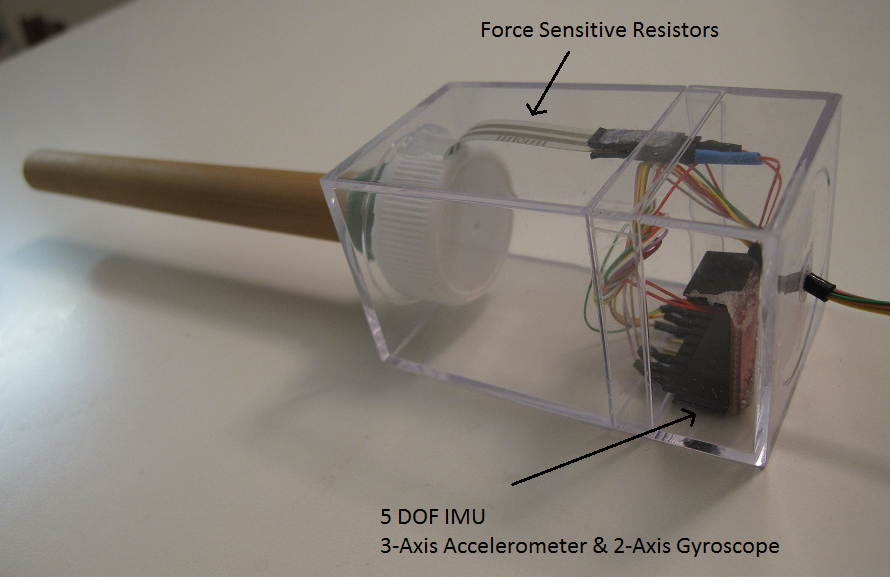
\includegraphics[width=\linewidth]{./figs/impl1.png}
  \caption{Our \tube with all the sensors.}
  \label{fig:impl1}
\end{figure}


We have developed two applications to demonstrate the interactivity of our \tube. The applications that we developed are written in processing since it provides a smooth interface with arduino while boasting numerous easy-to-use graphical functions. Making existing processing applications to work with our \tube require very minimal changes to the code base since we have made the interface to the hardware to be very simple and generic.

\subsection{\textbf{Painting Application}}

\marginpar{
\begin{figure}
  \begin{center}
  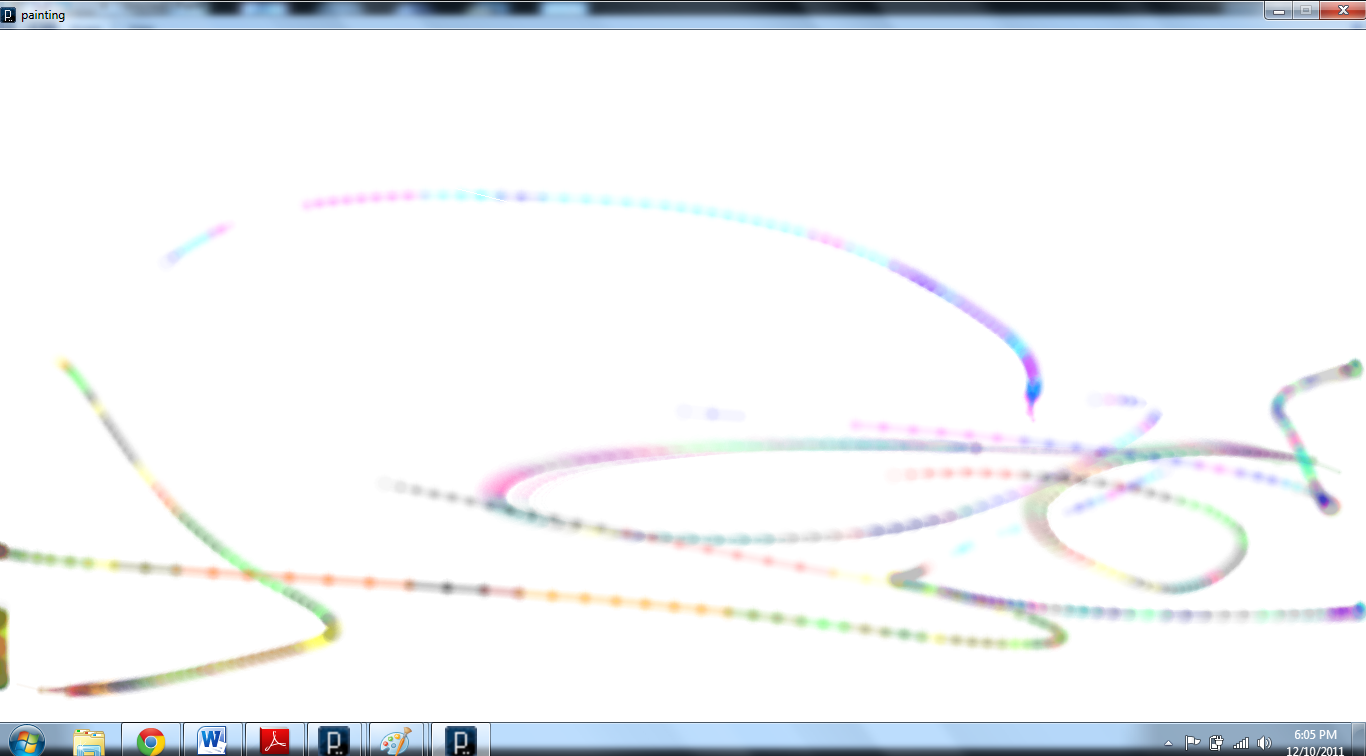
\includegraphics[width=\marginparwidth]{./figs/tube3.png}
  \caption{A screenshot of our painting application that one of the testers draws.}
  \label{fig:painting}
  \end{center}
\end{figure}
}

Our first application is a painting application program. In this application, the user will be able to paint by blowing into the tube and the harder the user blows, the thicker the color is. Changing the color of the paint is achieved by rotating the tube. We implement the paint to be brush-like and the color will disappear after a while to make it more like painting with a real brush.

\subsection{\textbf{Balloon Popping Game}}

The next application that we developed is a game in which the user is required to pass through a set of levels by shooting down balloons that randomly appear in the screen, as shown Figure~\ref{fig:shooting-game}. This is done by moving the pointer to where the balloons are and blow into the tube. The game consists of two levels: stage 1 and stage 2. In the first stage, the pointer and balloons color are always black so that users don’t have to rotate the tube to match the color. This stage is intended to familiarize the users with the basic concept on how to move the tube to control the pointer and use it to pop a balloon. The pointer is shaped like a circle and whenever the users blow the tube, there will be a spraying animation which size is determined by how hard the user blow. Every time a balloon is popped, the user will receive 1 point. After scoring a few points in the first stage, we take the users to stage 2 where the balloons are randomly generated with red, green, or blue color and the users will have to rotate the tube to change color of the pointer so that they can pop the balloon. When the game ends, users can simply blow the tube harder and it will take them back to stage 1. We also added a proper sound effects to make the game more engaging with the user.

\begin{figure}
  \centering
  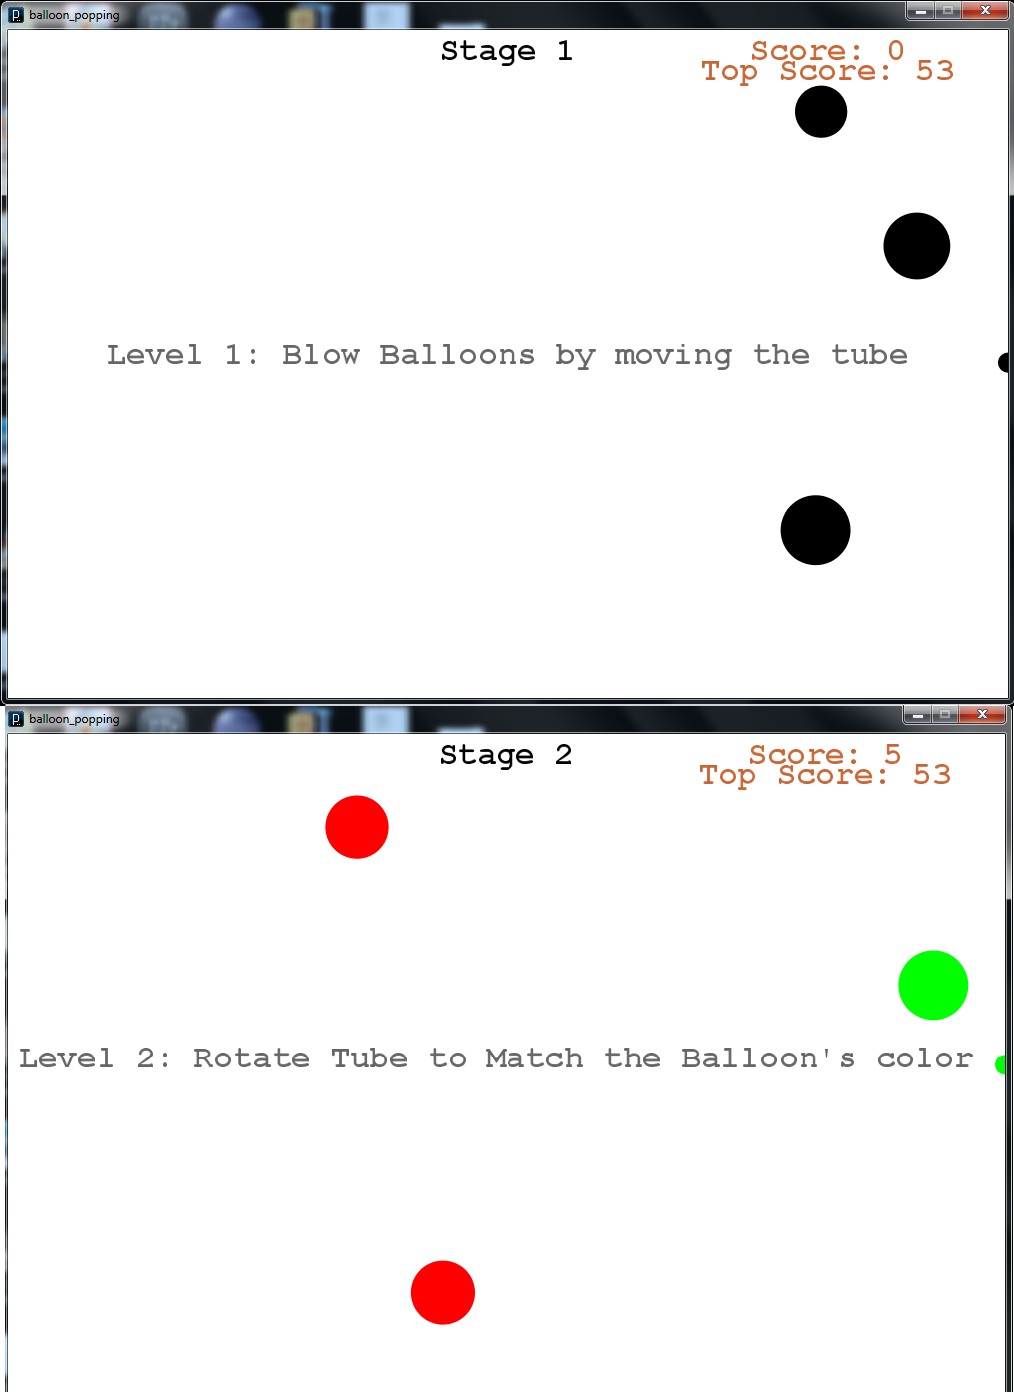
\includegraphics[width=0.8\linewidth]{./figs/tubemaster.png}
  \caption{A screenshot of the beginning of each level of our balloon popping game.}
  \label{fig:shooting-game}
\end{figure}

